\documentclass{article}
\usepackage[utf8]{inputenc}
\usepackage{caption}

\title{Advanced Quantum Theory}
\author{Tobias Osborne}
\date{Transcribed by Michael Astwood}
\usepackage{graphicx}
\usepackage{listings}
\usepackage{amsfonts}
\usepackage{amsmath}
\usepackage{MnSymbol,wasysym}
\usepackage{physics}
\usepackage{listings}
\usepackage{amsmath}

\DeclareMathOperator{\Col}{\textrm{Col}}
\DeclareMathOperator{\Nul}{\textrm{Nul}}
\DeclareMathOperator{\Bb}{\mathcal{B}}
\DeclareMathOperator{\Cc}{\mathcal{C}}
\DeclareMathOperator{\Hh}{\mathcal{Hh}}
\DeclareMathOperator{\Dd}{\mathcal{D}}
\DeclareMathOperator{\GL}{\textrm{GL}}
\DeclareMathOperator{\RR}{\mathbb{R}}
\DeclareMathOperator{\sgn}{\textrm{sgn}}
\DeclareMathOperator{\II}{\textrm{II}}
\DeclareMathOperator{\Ion}{\textrm{I}}
\DeclareMathOperator{\nul}{\textrm{null}}
\DeclareMathOperator{\RP}{\mathbb{RP}}
\DeclareMathOperator{\ZZ}{\mathbb{Z}}
\DeclareMathOperator{\CC}{\mathbb{C}}
\newcommand{\hk}{\mathbin{\! \hbox{\vrule height0.3pt width5pt depth 0.2pt \vrule height5pt width0.4pt depth 0.2pt}}}
\newtheorem{defn}{Definition}
\newtheorem{thm}{Theorem}
\begin{document}
\maketitle
\pagebreak
\tableofcontents

\pagebreak
\section{Introductions}
Instead of "Advanced Quantum Theory", you could call this course "From one to many". The principle goal of this course is to take the quantum mechanics of a single particle, and apply this quantum mechanics to the theory of many particles.
\subsection{Course Structure}
Assumed is knowledge about single-particle quantum mechanics: potentials, the hydrogen atom, harmonic oscillators, angular momentum, and so on. The books we will use in this course are as follows:
\begin{enumerate}
    \item \textit{Bratelli \& Robinson. Operator Algebras and Quantum Statistical Mechanics (Volume 2)}
    \item \textit{Taylor. Scattering Theory: The Quantum Theory of Nonrelativistic Collisions}
    \item \textit{Reed \& Simon. Methods of Modern Mathematical Physics (Volume 3: Scattering Theory)}
    \item \textit{Weinberg. Quantum Theory of Fields (Volume 1: Foundations)}
    \item \textit{Leinhaas \& Myrheim. On the Theory of Identical Particles}
\end{enumerate}
\begin{center}\fbox{\parbox{\textwidth}{
Course Outline
\begin{enumerate}
    \item Identical Particles
    \begin{enumerate}
        \item Classical Case
        \item Quantum Case
        \item Second Quantization
        \item Canonical Commutation Relations (CAR/CCRs)
    \end{enumerate}
    \item Scattering Theory
    \begin{enumerate}
        \item In/Out States
        \item Moeller Spaces
        \item S-Matrices
        \item Green's Operators, T Operators
        \item Stationary Scattering States
    \end{enumerate}
    \item Relativistic Quantum Mechanics
    \begin{enumerate}
        \item Quantum Lorentz \& Poincare Transformations
        \item Wigner's Theorem
    \end{enumerate}
\end{enumerate}
}}
\end{center}
\pagebreak
\subsection{Motivation}
In order to understand how to approach moving from a theory of single particles to a theory of many particles, it is important to understand the way in which physical quantum theories are developed. Figure 1 is a representation of how these theories are built. Consider the space of quantum theories (for the purposes of this, a quantum theory is a pair $\{\mathcal{H},\hat H\}$). Each of these theories has a space of states, $\Hh$, and an observable called a Hamiltonian ($\hat H$) which governs the dynamics of those states. When we measure these systems in real life, we are limited by our measurement apparatus. The objects we measure are subject to decoherence, and the apparatus is imperfect, and so through decoherence and imperfect measurement we end up observing something called a "classical limit", which corresponds to one of the many classical theories in the space of classical theories. A classical theory, similarly to a quantum theory, is given by a pair $\{\mathcal{M},H\}$ of a manifold (or some other topological space) $\mathcal{M}$ called the phase space along with the classical Hamiltonian $H$ governing the dynamics of the system. Quantization is the process of reversing this classical limit - we would like to take $\{\mathcal{M},H\}$ and find some $\{\mathcal{H},\hat H\}$ which matches the theory. The issue with this is that this process is not well posed - many quantum theories can describe the same classical limit, and we will see examples of this in the course. In order to simplify this task, one of the major tools at our disposal is symmetry! We would expect a quantum theory to have the same symmetries as the classical theory, so narrowing the potential quantum theories down to the ones with these properties is helpful when quantizing a theory. One of the most important symmetries for this course is the symmetry of particle exchange, and that's where we will commence this course.\footnote{For a comprehensive description of "quantization" as a process, see Ali and Englis' review paper on the topic. This course will only cover the Canonical Quantization method in detail, but there is still more to learn in Canonical Quantization as well}
\begin{figure}[ht]
    \centering
    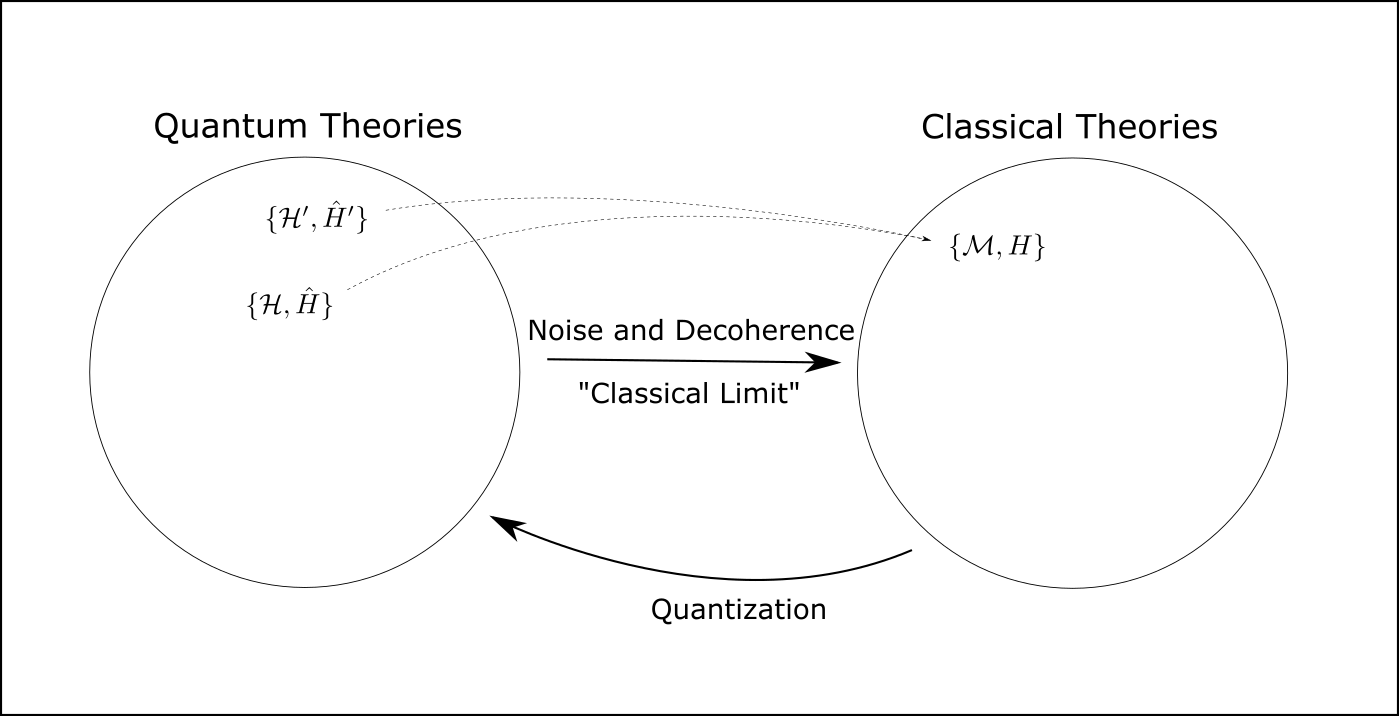
\includegraphics[width=\linewidth]{Figures/fig1.png}
    \caption*{}
    \label{fig:fig11}
\end{figure}
\pagebreak

\subsection{Classical Theory of Identical Particles I}
Why do we want to develop a (classical) theory of identical particles? The answer comes in the form of the Gibbs Paradox. The Gibbs Paradox says that if you have an ideal gas in equilibrium in a container, and you place a barrier into the container, the entropy decreases. This would be bad, because you'd be well on your way to breaking the 2nd law of thermodynamics, and infinite wealth, fame, and glory awaits you. (Un)fortunately, this paradox is resolved if the particles are \textit{indistinguishable}. So first of all, why bother studying these systems of identical particles in any more depth? The answer is that they give us an intuition about what to expect our classical limit to look like. Secondarily, there are many interesting structures that come out of these systems.

Let's begin with a system of $N$ identical classical particles. One's intuition might guess that the phase space of this system is simply the direct product of the individual phase spaces. Let $X$ be the configuration space of this system, and $X_i$ is the configuration space of some $i$'th particle. Then our intuition would tell us that $X = X_1 \times ... \times X_N$. Let $\pi \in S_N$ (where $S_N$ is the symmetry group on $N$ symbols). Then there is no way to distinguish each state $x = (x_1,...,x_N) \in X$ from $x' = (x_{\pi(1)},...,x_{\pi(N)})$ since the particles are identical!  To clarify, we have the following:
\begin{align*}
    x &= (x_1,...,x_N) \\
      &= (x_{\pi(1)}, ... , x_{\pi(N)})
\end{align*}
Let $x, y \in X$. Then we will define an equivalence relation on $X$ given by $x \sim y$ if $(x_1,...,x_N) = (y_{\pi(1)},...,y_{\pi(N)})$. The true configuration space of $N$ particles moving in some system $X$ should therefore be given by the following quotient:
\[\mathcal{M} \equiv X^N / \sim\]
Recall that the elements of a quotient space are the equivalence classes, that is: each element is given by $[x] \equiv \{y | y \sim x\} \in \mathcal{M}$. Typically we abuse notation and write $x = [x]$. If you know about topological spaces, you should by now be saying "uh oh", because quotients do strange things to topological spaces. One of the things a quotient does to a nice topological space is introduce a singularity in the space. We will see this soon. Let's take a simple example: if $X = \RR^n$, then as $S_N$ is a finite group, $\mathcal{M}$ is locally diffeomorphic to $(\RR^n) \times ... \times (\RR^n)$ ($N$ times). What this means is that if you have $N$ particles far away from each other, then it's as if you can look at each particle on it's own. The interesting things happen when particles are near each other, and that's when you get so-called 'singularities'. So let's look at the simplest example we can come up with. $X = \RR$, and $N = 2$.
\pagebreak
\begin{figure}[ht]
    \centering
    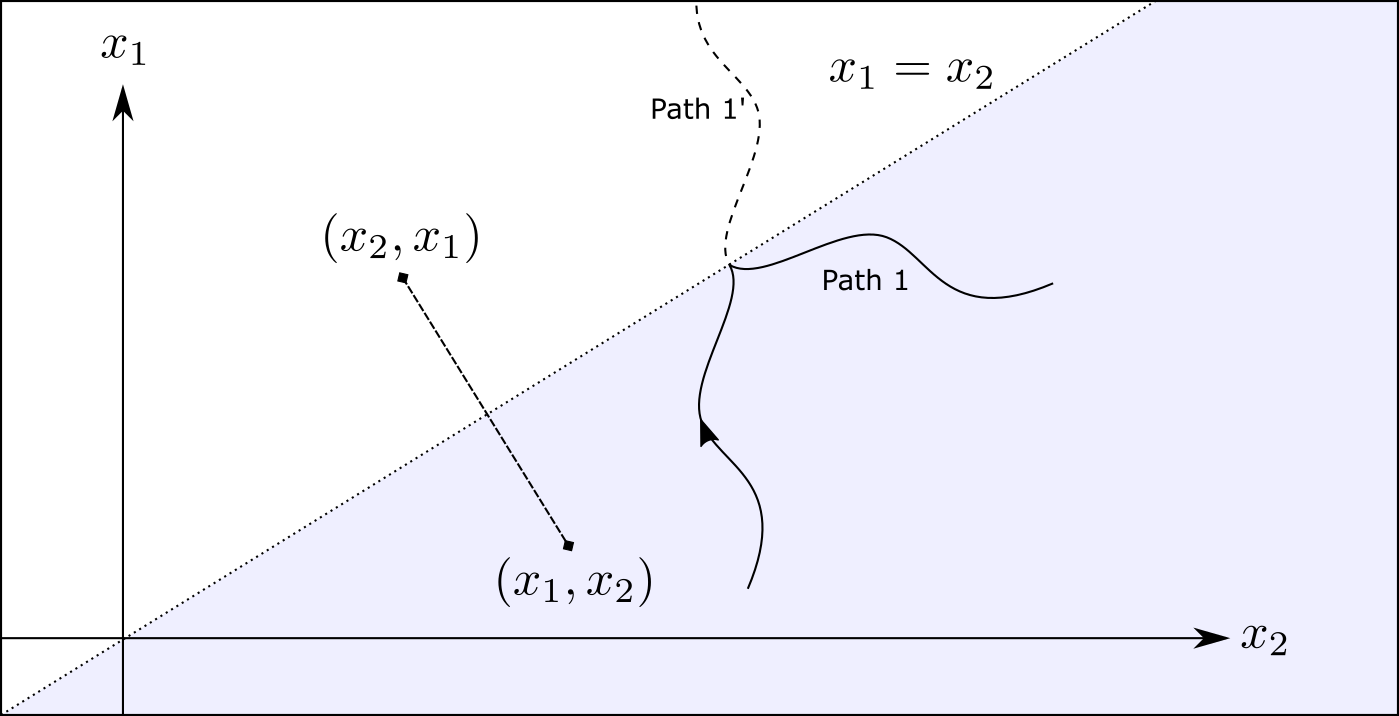
\includegraphics[width=\linewidth]{Figures/figure2.png}
    \caption*{}
    \label{fig:fig12}
\end{figure}

We are going to choose for our representatives of $\mathcal{M} = \RR^2/\sim$ to be the ones given by $x_1 < x_2$. Then an embedding of $\mathcal{M}$ in $\RR^2$ is given by the region $\{(x,y):x<y\}$.

Above is a diagram of our space $\mathcal{M}$ (in blue, embedded in $\RR^2$). We see that in this space, $(x_1,x_2)$ is identified with $(x_2,x_1)$ as $1\mapsto 2$, $2\mapsto 1$ is the only permutation on $\RR^2$. You can see that any point in the interior of the space (completely surrounded in blue) is going to be the same as if it were just in $\RR^2$ - this is what we mean by locally diffeomorphic.


Any path in $\RR^2$ which attempts to cross the line $x_1=x_2$ is going to have something strange happen to it - the path actually reflects, and rather than Path 1' we get Path 1. If you look closely, a tangent vector to the curve undergoes a (discontinuous) reflection when it touches the boundary. This is some interesting behaviour, and demonstrates that our spaces are going to have non-trivial features.
Generally, if $X = \RR^n$ we are going to introduce the center of mass coordinates. If we are in units where each particle has mass $m=1$, then we choose the following:
\[x_{cm} = \frac{1}{N}\sum_{i=1}^N x_i\]
This gives us the result that $\pi(x_{cm}) = x_{cm}$ for any $\pi \in S_N$. What this allows us to do is set $\mathcal{M} = \RR^n \times r(N,n)$, where $r(N,n)$, the \textit{relative space}, encodes the strange global effects we observe of our space, and $\RR^n$ encodes the local information about the space. It turns out that $r(N,n)$ is some $n(N-1)$ dimensional space, but it is not necessarily a differentiable manifold (this is an example of something called an \textit{orbifold}). Now that we have seen the case of $n=1, N=2$, we can move on to arbitrary $n$. Let's analyze the structure of this relative space $r(2,n)$. Let $x_1$ and $x_2$ be the configurations of two particles in $\mathcal{M}$. For our equivalence relation, if we identify $x = x_1 - x_2$ with $-x = x_2 - x_1$, we see that there is one singular point at $0$. In fact, since the equivalence relation simply provides the distance between the two particles in this space as a nice representative, we will see in a second that $r(2,n) \setminus \{0\} = \RR^{+} \times {\RP}^{n-1}$. In general, the section given by $\RR^+$ provides the 'length' of the relative coordinate $x$ (which is why it's called a relative space - this is the distance between the particles), and the other part is something called the real projective space. The simplest examples are $\RP^0$, which is a point, and $\RP^1$, which is a circle. But when $n\geq 3$, $\RP^n$ is a \textit{doubly connected} space, meaning that any closed curve with winding number 2 around the singularity is contractible. The fact that this space is doubly connected (in three dimensions) is important! It will later provide two options for the configuration of a particle, which in turn provides us with two types of particles which we call fermions and bosons. On the other hand, in two dimensions the consequence of $\RP^1$ being a circle is that since the circle is not simply connected, there are interesting phenomena that happen when particles are constrained to move in two dimensions.

Here's a more specific example. Consider two particles moving in $\RR^2$. Then we have $\mathcal{M} = (\RR^2)^{\times 2}/\sim = \RR^2 \times r(2,2)$. It is an exercise to show that $r(2,2)$ is the same as the plane $\RR^2$ with the origin removed and where $x$ is identified with $-x$ (that is, $r(2,2) = \RR^2 / a$, where $a$ is the antipodal map). Below is a rather unsatisfying drawing of this space. You can imagine the bottom of the cone as being the origin. The way that the cone wraps around itself indicates how at each point on the cone, two points of $\RR^2$ are represented - the inside being the negative values and the outside being the positive values.
\begin{figure}[ht]
    \centering
    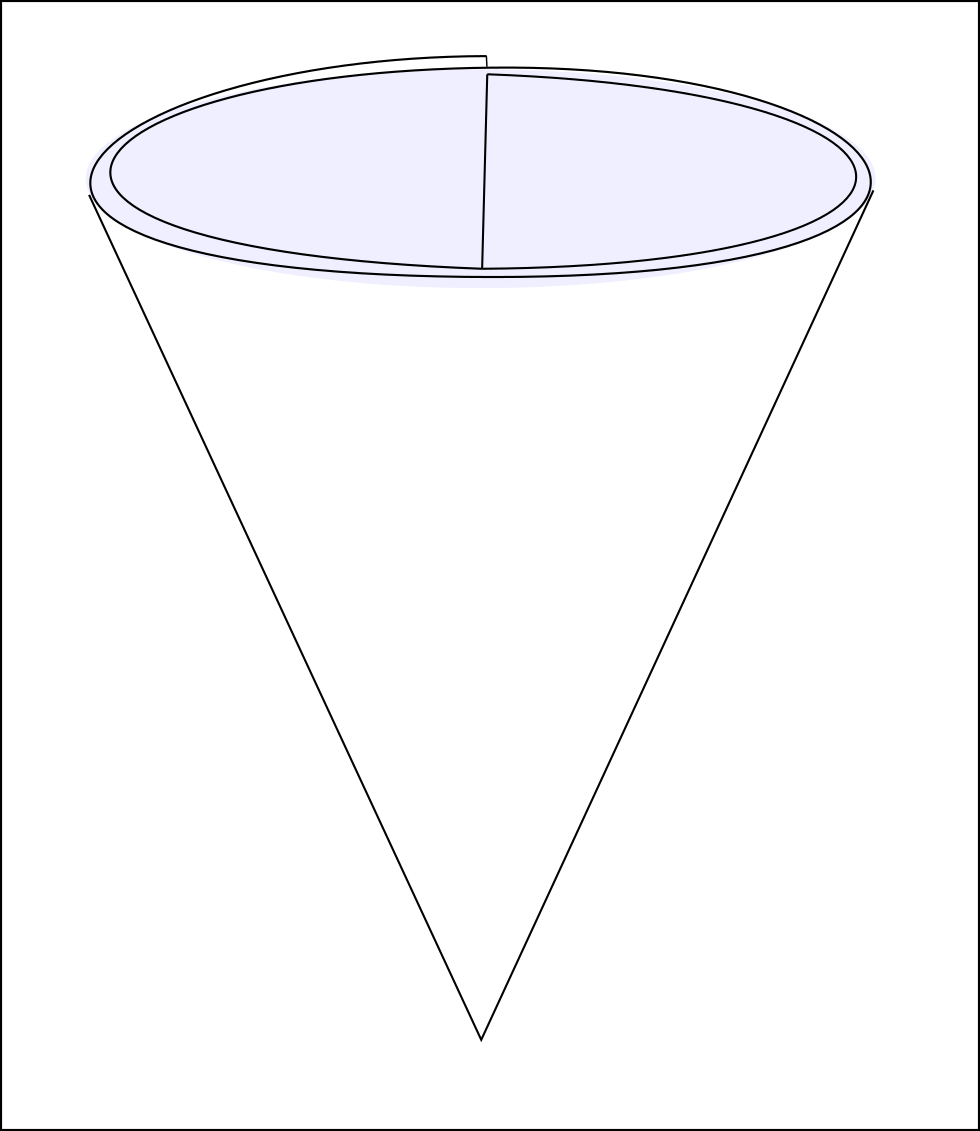
\includegraphics[width=0.5\linewidth]{Figures/rp1.png}
    \caption*{}
    \label{fig:my_label}
\end{figure}
\pagebreak
\section{Relative Space and Quantization}
\subsection{Classical Theory of Identical Particles II}
We noticed in the last section that given a configuration space $\mathcal{M} \equiv (\RR^n)^{\times N}/\sim$, we could rewrite the space in the center-of-mass coordinates to find that $\mathcal{M} = \RR^n \times r(N,n)$, where $r(N,n)$ looks locally like $\RR^{n(N-1)}$ but with a few nasty extra features. The difference between the two manifests in the global (topological/geometric) properties of the spaces. Particularly in the analysis of \textit{parallel transport} and \textit{tangent vectors}. Though we haven't talked in detail about what a tangent vector is, for now we can use our intuition about velocity vectors - it is a vector valued object defined at each point along some curve or surface, and in this particular case we require the vector to be in some sense 'tangent' to the surface. You will see these notions defined in more detail in courses on general relativity or differential geometry, and the geometry of configuration spaces is very closely related to what we call 'gauge theories', which you will see later on as well. If you would like the full picture, it would be beneficial to spend some time studying what is called the \textit{tangent bundle} of a manifold.

\subsubsection{Tangent Vectors}

Let's now use our intuition about velocity to consider some configuration spaces. We say that a velocity vector $v$ is a 'tangent vector to the configuration space', meaning that there is some curve through $\mathcal{M}$ which has velocity $v$ at some point $x$. As an example, in $\RR^2$ a particle requires both position and velocity in order for you to fully specify its' state - we therefore say that the \textit{state} of the particle is the pair $(x,v)$. In a simple space such as $\RR^2$, comparing the velocities of particles is simple, but we often take for granted the process of adding vectors 'tip to tail'. This way of comparing velocities is where you take the velocities as vectors in $\RR^2$ and subtract them pointwise. This works in $\RR^n$ easily, but you have to be more careful when considering so-called 'tangent vectors', which exist in a more complicated space called the tangent space. The tangent space is defined separately at each point in the 'ambient space' (here being \textrm{M}). For $\RR^2$, this is simply $\RR^2$ everywhere. But for an arbitrary manifold $\mathcal{M}$, the tangent space may be different at each point. Therefore we would like a way to transport velocities between tangent spaces in a continuous/parallel way. This is called parallel transport.
\pagebreak

\begin{figure}[ht]
    \centering
    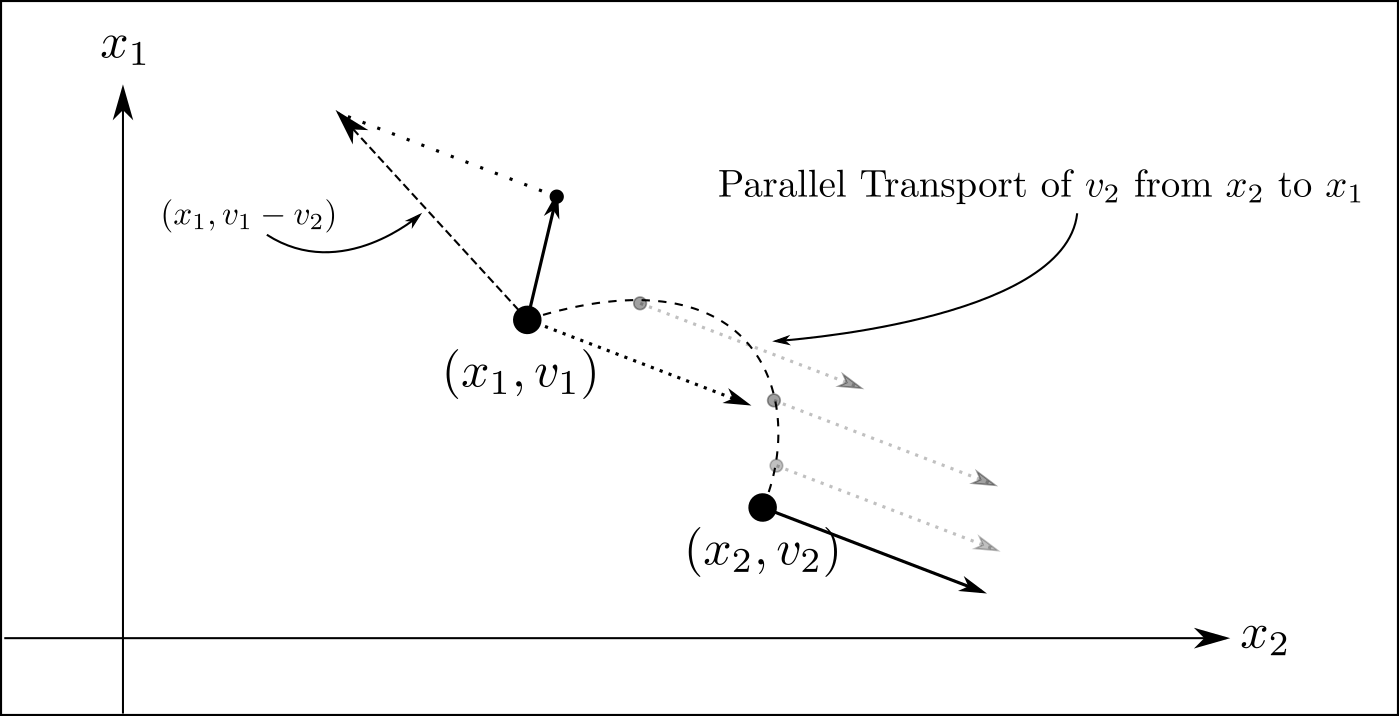
\includegraphics[width=\linewidth]{Figures/figure3.png}
    \caption*{}
    \label{fig:21}
\end{figure}
The above diagram demonstrates this notion of parallel transport in $\RR^2$. Luckily, in euclidean space it does not matter what path we transport $v_2$ along. But there is a simple example where parallel transport fails! Imagine a curve which goes from some point to the north pole, changes direction, comes back down to the original latitude, and goes back to its' origin. A diagram will help.
\begin{figure}[h]
    \centering
    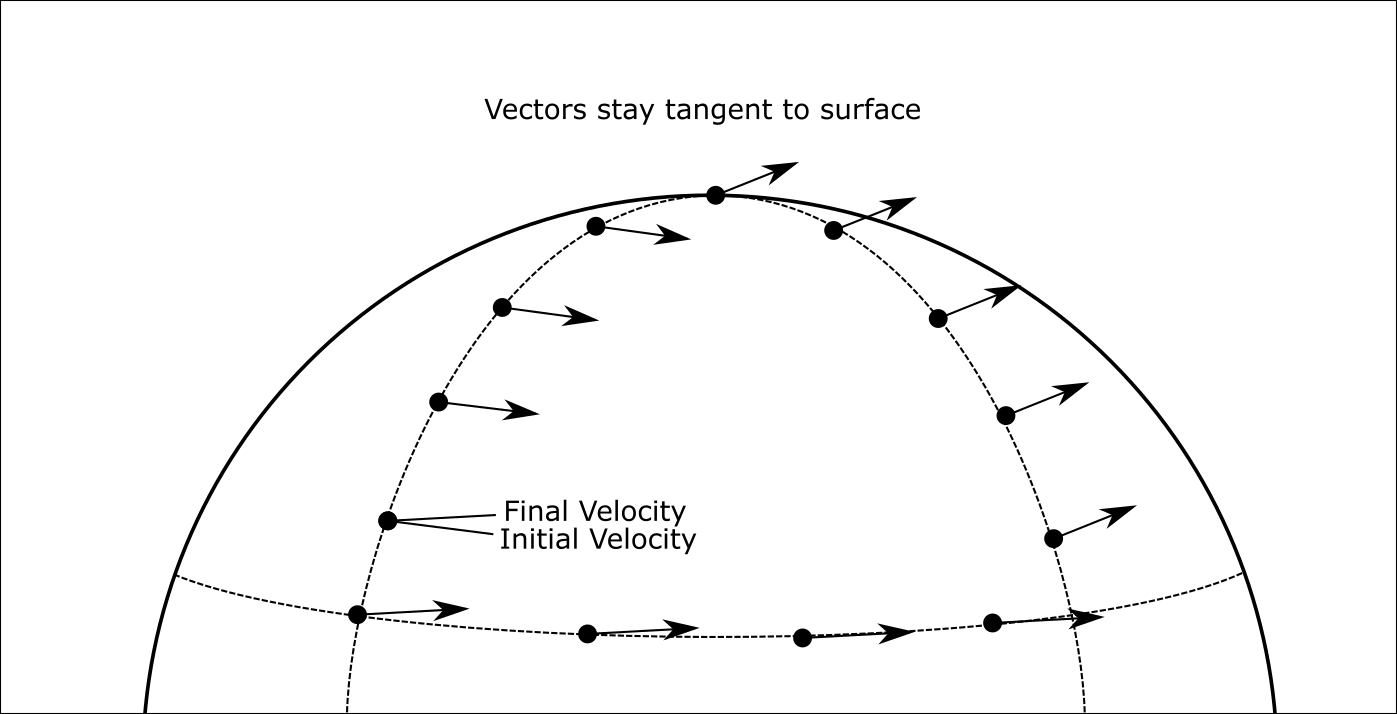
\includegraphics[width=\linewidth]{Figures/spheretransport.png}
    \caption*{}
    \label{fig:22}
\end{figure}

You will notice that if you draw vectors which \textit{stay tangent to the surface of the sphere}, then they change direction slightly as you move across the surface of the sphere. A vector (as shown in the diagram) which starts tangent to a line of latitude will eventually end up being perturbed by the motion.
\pagebreak

\subsubsection{Parallel Transport in Relative Space}
Let's consider this parallel transport in our relative space $r(2,2)$, which we saw earlier could be represented as that sort of 'cone' shape. You can check that on an ordinary trajectory on the surface of this cone, vectors do not undergo any strange transformation. But consider when a vector is transported around the singularity. Suppose the trajectory begins at a point $x$, and crosses through the point $-x \sim x$. A vector held parallel along this trajectory is going to have to undergo the transformation $v \mapsto -v$ in order to satisfy the criteria for 'parallel transport'. You can see the reasoning behind this in more detail in any text on Differential Geometry.

Now let's look at three dimensions. We consider the relative space $r(2,3) \cong \RP^2$ of two particles living in three spacial dimensions. A good way to visualize this space is as follows. Imagine the sphere, where each point $x$ is identified with the point on the opposite side of the sphere. As you move towards the equator, you need to identify points on opposite sides of the equator. In this way, it's sort of like the upper half of the sphere (of radius $d/2$, where $d$ is the distance between the particles). There are some great visualizations of this on wikipedia, if you look up 'real projective space'.

The next thing to do would be to try to look at trajectories in this space, so let's consider a few different trajectories, as shown in the next figure.

\begin{figure}[h]
    \centering
    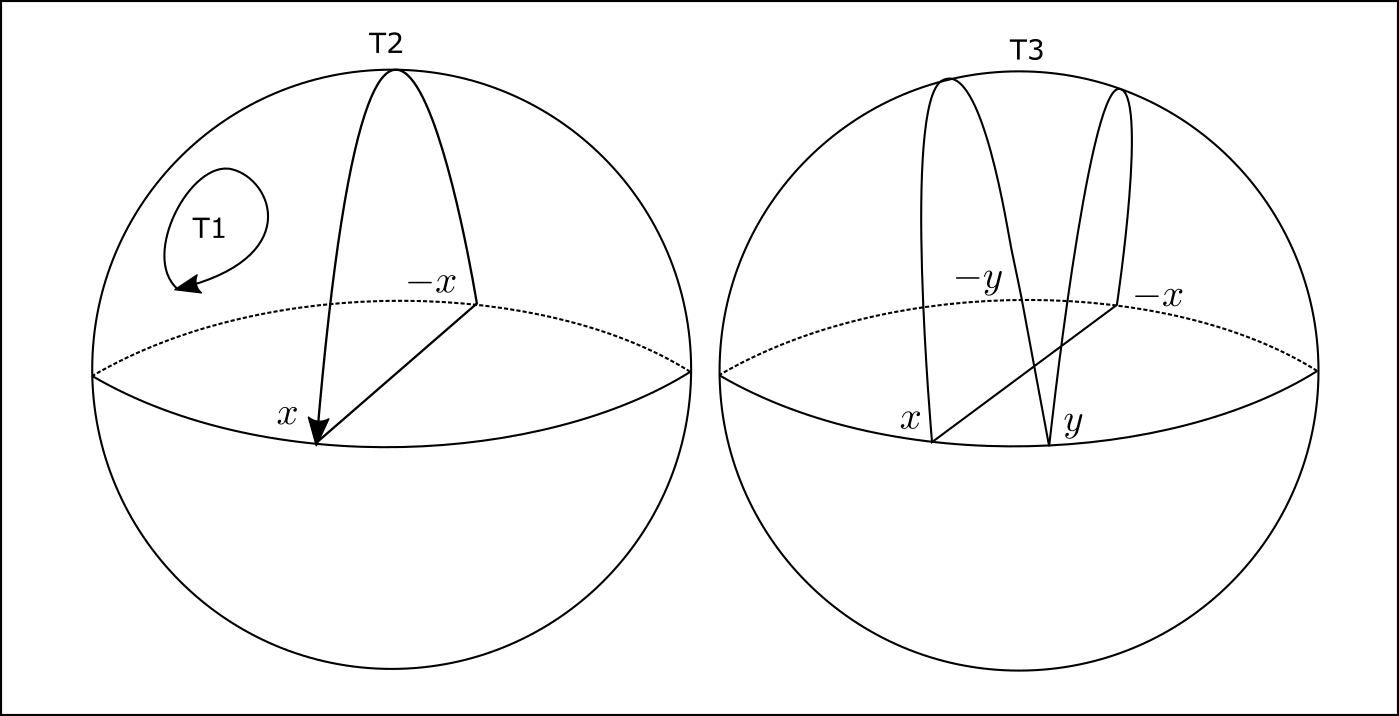
\includegraphics[width=\linewidth]{Figures/trajectories_in_rp2.png}
    \caption*{}
    \label{fig:23}
\end{figure}

The trajectory T1 is contractible to a point, as this region is clearly simply connected. The trajectory T2 begins at a point on the equator, moves over the surface of the sphere, and then returns to the 'same' point on the other side of the sphere, and the trajectory T3 follows a similar path. It turns out that T3 is contractible to a point, but T2 is not! The reason for this is that T3 passes around the singularity twice, whereas T2 only passes around the singularity once. A space like this is called \textit{doubly connected}, and can be studied in detail in a Topology course. 

Now, why did we spend so much time going over these weird properties? I hope this sets the stage for the study of the mysterious properties of these configuration spaces, but these properties don't have much of an effect in classical mechanics. This is because classical mechanics is very local. The place where this becomes much more important is in quantum systems. So we are now going to leave the topic of classical particles, and begin the study of quantum point particles.

\subsection{Quantization of Identical Quantum Particles I}

We need to remember that the problem of quantization is not very well posed. Many quantum systems can result in the same classical system, so we need to consider some guiding principles. As as example, if our configuration space $\mathcal{M}$ is continuous, we should take $L^2(\mathcal{M})$ as our Hilbert space - this is a very common approach. But we know that this is just one example of a probabilistic theory - there are quite a few structure that could give the same probabilistic data for a system, so we need to answer a specific question: \textbf{What do we mean by wavefunction?} A very literal approach would be that a wavefunction is a function! 
\[\Psi: \mathcal{M} \to \CC\]

But there is an alternative interpretation to the word wavefunction, and it can give inequivalent results! Let's construct it. First we need to build some space $E$ which is locally similar to $\mathcal{M} \times \CC$ (it could just be $E \cong \mathcal{M}\times \CC$). As an example, we could take $\mathcal{M} = \RR$. A trajectory in $E \cong \RR \times \CC$ would be equivalent to what you've learned in single particle 1D quantum mechanics - below is a diagram of what this looks like. But this construction becomes different when you start looking at spaces which have singularities and other strange properties. So let's put some terminology together.

The space $\mathcal{M}$ is called the \textit{base space}. The space $\CC$ is called the \textit{fibre}. The space $F$ is called the \textit{fibre bundle}, and a choice of an element in $\CC$ for each point in $\mathcal{M}$ is called a \textit{section}. Since our fibre is $\CC$, we will just call this a $\CC$-bundle.

\begin{defn}[Vector Bundle]
Let $\mathcal{M}$ be a manifold. Suppose for each point $x \in \mathcal{M}$ we associate a vector space $h_x$. We define a vector bundle over $\mathcal{M}$ to be the disjoint union $\sqcup_x h_x = E$. This definition provides the existence of a projection $\pi : E \to \mathcal{M}$ given by $\pi(x,h_x)=x$.
\end{defn}


\begin{defn}[Section]
	Suppose $E$ is a vector bundle over $\mathcal{M}$. A section of $E$ is a map $\Psi : \mathcal{M} \mapsto h_x \in E$, so that $\Psi(x) = \psi(x)\chi_x$. The set of all sections of $E$ is denoted $\Gamma(E)$.\footnote{In the case $E=T\mathcal{M}$ (the tangent bundle), we write $\Gamma(TM) = \mathfrak{X}(M)$}
\end{defn}

\begin{defn}[$\CC$-Bundle]
	A $\CC$-bundle over a manifold $\mathcal{M}$ is a vector bundle $E$ where each $h_x \in E$ has $h_x \cong \CC$.
\end{defn}

So that's one interpretation of a wavefunction - it's a section of a $\CC$-bundle over a base space $\mathcal{M}$ (provided the section meets some continuity and differentiability requirements, which won't be discussed in depth). Why go through these complicated constructions with all this terminology? Because there are sometimes multiple nontrivial $\CC$-bundles over a space which are \textit{inequivalent}! We can even go further, as a nice example we can consider relatively simple spaces over which there are inequivalent $\RR$-bundles (fibre bundles where the fibre is $\RR$). We could consider "real" quantum mechanics, where every wave function is real-valued. There are some problems with the theory of real quantum mechanics (mostly with entanglement), but it's a perfectly respectible theory in many ways. So consider the base space $\mathcal{M} = S^1$, the circle. We will construct two different $\RR$-bundles over the circle, which are shown on the following page in a diagram from the Encyclopedia Britannica.

\begin{figure}[h]
    \centering
    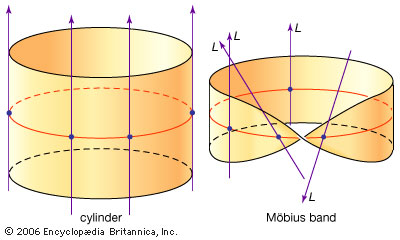
\includegraphics[width=\linewidth]{Figures/mobius_bundle.jpg}
    \caption*{}
    \label{fig:24}
\end{figure}

In order to describe wavefunctions as sections of these bundles, it's therefore important to consider the vector space properties of $\CC$, as you could choose some basis vector for the fibre and it will twist and turn as you move around the base space. The way we do this is to further generalize our fibre bundle. Let's just consider our base space $\mathcal{M}$, and for each point $x$ in $\mathcal{M}$ we will associate a fibre $h_x$. In our case, we will always be using $\CC = h_x$, but it's important to make this generalization so that we can write the following. We want to make some choice of (normalized) basis vector $\chi_x$ for each $h_x$, so that $\textrm{Span}(\chi_x) = h_x$. Thus any section $\Psi$ can be written so that you can evaluate $\Psi$ at a point: $\Psi(x) = \psi(x)\chi_x$. You could therefore change this basis vector as you move around the space! Such a choice of $\chi_x$ for each $h_x$ is called a choice of gauge, and it's the same gauge you refer to in gauge theory. Suppose you wanted to change your basis vectors, so that $\chi_x \mapsto e^{-i\varphi(x)}\chi'_x$. Then you'd require that $\psi'(x) \mapsto e^{i\varphi(x)}$ so that $\Psi$ is unchanged. This is called a gauge transformation. The fact that physical quantities should not depend on this choice of gauge (gauge invariance!) causes issues when defining your derivative operator, and we will talk about this in the next section.

\pagebreak
\section{Identical Particles: Foundations}
\subsection{Quantization of Identical Quantum Particles II}
We won't spend too long talking about the theory of $\CC$ bundles. In this lecture we will move towards understanding identical particles, types of identical particles, and how to describe them in quantum mechanics. Today is the last day we will talk about understanding how there can be more than one quantization for a given classical system, due to this description in terms of $\CC$ bundles. So let's get into it. Here's some recap of the previous section.

Recall that a \textbf{State} is an assignment of complex vectors at each point in $\mathcal{M}$, or in other words, it is a section of a $\CC$-bundle over $\mathcal{M}$. To do computations with this on a computer, we need to choose a basis for each point in the $\CC$-bundle. Such a choice of basis is called a \textit{frame}.

\begin{defn}[Frame]
	Given a fibre bundle $E$, A \textit{local frame} for $E$ on some open set $M \subseteq \mathcal{M}$ is a choice of basis $\chi_x$ for each $h_x \in E$, with $x \in M$.
\end{defn}

\begin{defn}[Quantum State]
	A state $\Psi(x)$ of a quantum system is a \textit{section} of a $\CC$-bundle over the configuration space $\mathcal{M}$ of the system.
\end{defn}

Let $h_x$ be the fibre at the point $x \in \mathcal{M}$. Then we can choose a normalized basis vector for $h_x$ denoted $\chi_x$. Recall that for $\RR$ we can only choose $1$ or $-1$ to be our normalized basis vectors, but in $\CC$ we can choose $e^{i\phi}$ to be our normalized basis vector.

Once we've chosen this basis $\chi_x$ then we could write $\Psi(x) = \psi(x) \chi_x$.

We want to understand how to keep our quantities invariant to our choice of basis. So let's recall the \textit{Gauge Transformations}, which are transformations of the form $\chi'_x = e^{-i\phi(x)}\chi_x$. Under a gauge transformation, $\Psi$ is transformed by $\Psi'(x) = \Psi(x) \exp(i\phi(x))$. The clear example of a gauge invariant quantity is the probability amplitude $\overline{\Psi(x)}\Psi(x) = p(x)$. This is expected. But we'd also like to look at other quantities, such as our position and momentum operator.

\begin{defn}[Gauge Transformation]
	A gauge transformation $U$ is a choice of maps $U_x : h_x \to h_x$ with $U_x(\chi_x) = e^{-i\phi(x)}\chi_x$. This induces a transformation on sections of $E$ as so: $U[\Psi](x) = e^{i\phi(x)}\Psi(x) $
\end{defn}
\pagebreak

\subsection{Making Momentum Gauge Invariant}

Let's try to show that the momentum operator (that we learned about originally) is not gauge invariant. Recall that (in natural units) $\hat p = -i \pdv{x^k}$

\[\hat p \Psi' = -i \lim_{\epsilon \to 0}\frac{e^{i\phi(x+e_k\epsilon)}\Psi(x+e_k\epsilon) - e^{i\phi(x)}\Psi(x)}{\epsilon}\]

As we can see $\phi(x+e_k \epsilon) \neq \phi(x)$, and in the limit as $\epsilon \to 0$ it is not guaranteed that they are equal! We didn't require that $\phi$ be continuous. What this means is that we could set up an experiment to measure $\phi$ and recieve information about gauge, which means that this formulation is not independent of our choice of basis. The next step is to therefore develop a new notion of momentum.

\subsubsection{Using Parallel Transport}

As we saw in the previous section, parallel transport provides a nice way of comparing two tangent vectors (in this case the gauge $\chi_x$) in order to develop a new difference quotient. Let's look more closely at the precise definition of parallel transport. 

Recall that to parallel transport a vector in a tangent space $h_x$ into a different space $h_y$. Therefore we'd like a map (preferably a linear one!) that transports these vectors. This map will of course depend on the path $\gamma(t)$ between $x$ and $y$, and we will denote it $P_\gamma(y,x)$\footnote{This map will also often be denoted $\Gamma(\gamma)_x^y$, for example on wikipedia.}.

\begin{defn}[Parallel Transport Map] The parallel transport map is a linear map $P_\gamma(x,y) : h_x \to h_y$, with the following additional properties.
\begin{itemize}\setlength\itemsep{0.5em}
\item$ P_\gamma(x,x) = \mathbb{I}$
\item$ P_\gamma(y,z) \circ P_\gamma(z,x) = P_\gamma(y,x)$
\item$ P_\gamma(y,x)$ is an isomorphism (with $P_\gamma(x,y)=P^{-1}_\gamma(y,x)$)
\end{itemize}
\end{defn}
 
We would like $P_\gamma(y,x)$ to be gauge invariant so that the following holds:

\begin{equation}
P_\gamma(y,x) \mapsto e^{-i\phi(y)}P_\gamma(y,x) e^{i\phi(x)}
\end{equation}

We would also like to see that $P_\gamma(y,x) \to \mathbb{I}$ as $y \to x$ as long as $\gamma$ is a sufficiently well behaved path (that is, it's the most "direct path" between the two points) \footnote{a minimal geodesic}. In other words, $P_\gamma(x+dx,x) \approx \mathbb{I} - i \dd x^k b_k(x)$, where $b_k$ are the relevant taylor expansion coefficients. 

\pagebreak

This discussion of parallel transport leads us to our next definition, the covariant derivative. This is a method of differentiating vector fields (ie, sections of vector bundles) which leaves the structure of a manifold intact.

\begin{defn}[Covariant Derivative]
Let $\mathcal{M}$ be a manifold with $\CC$-bundle $E$. Suppose there is a suitably well behaved parallel transporter $P$ on $E$, and that $\Psi \in \Gamma(E)$. The covariant derivative in the direction of $e^k$ is denoted $D_k$ and is defined as follows.
\begin{align}
D_k \Psi(x) &= \lim_{h \to 0} \frac{P_\gamma (x,x+h e^k) \Psi(x+he^k) - \Psi(x)}{h}\\
	&= \lim_{h \to 0}\frac{(\mathbb{I} - i h e^k b_k(x))\Psi(x+ he^k) - \Psi(x)}{h}\\
	&= \left[\pdv{x^k}-ib_k(x)\right]\Psi(x)
\end{align} 
\end{defn}

Some exercises are as follows. First determine how $b_k(x)$ transforms under a gauge transformation. Then show that $D_k$ is gauge invariant. Third, show that for a single particle with spin, the Hamiltonian $\sum_k \frac{-1}{2m} D_k^2 = H$ is equivalent to that given by a static magnetic field (this tells us how such geometric changes could be induced experimentally). In the end, you will learn that these $b_k(x)$ are similar to the choice of magnetic field - they are related to the gauge field $A$.

The issue with this is that we want particles to locally behave like free particles - we don't want particles on their own in the middle of nowhere to act as if they are in magnetic fields. So we need to choose $b_k(x)$ so that the 'ficticious' magnetic force is zero. For nontrivial geometries, there do exist choices of $b_k(x)$ so that the force field will vanish (that is - the curvature tensor associated with the ficticious field vanishes). You may recall this expression from electrodynamics (it essentially says that $A$ is curl-free, or that $B=0$).

\begin{equation}
f_{k\ell}(x) = i[D_k,D_\ell] = \pdv{b_\ell}{x^k} - \pdv{b_k}{x^\ell}=0
\end{equation}

As long as equation 5 is imposed everywhere (except singularities, such as is the case on $\mathcal{M}=r(2,2)$) we will have freedom in choosing the $b_k$ terms. This freedom at the singularities allows us to pick nontrivial $b_k$ terms, which gives rise to interesting phenomena in 2-d materials. Due to $b_k$ being curl free, we also now know that $P_\gamma(y,x)$ is path independent as long as $\gamma$ does not encircle the singularity.

Let's study what happens when you go in a loop around the singularity. You can see that $P_\gamma(x,x)$ should just be some number $e^{i\xi}$ for some $\xi \in [0,2\pi)$, as $h_x \cong \CC$ and $\dim(\CC)=1$. However, this $\xi$ turns out to be independent of $x$! To demonstrate this, see the followng figure. 

\pagebreak

\begin{figure}[ht]
    \centering
    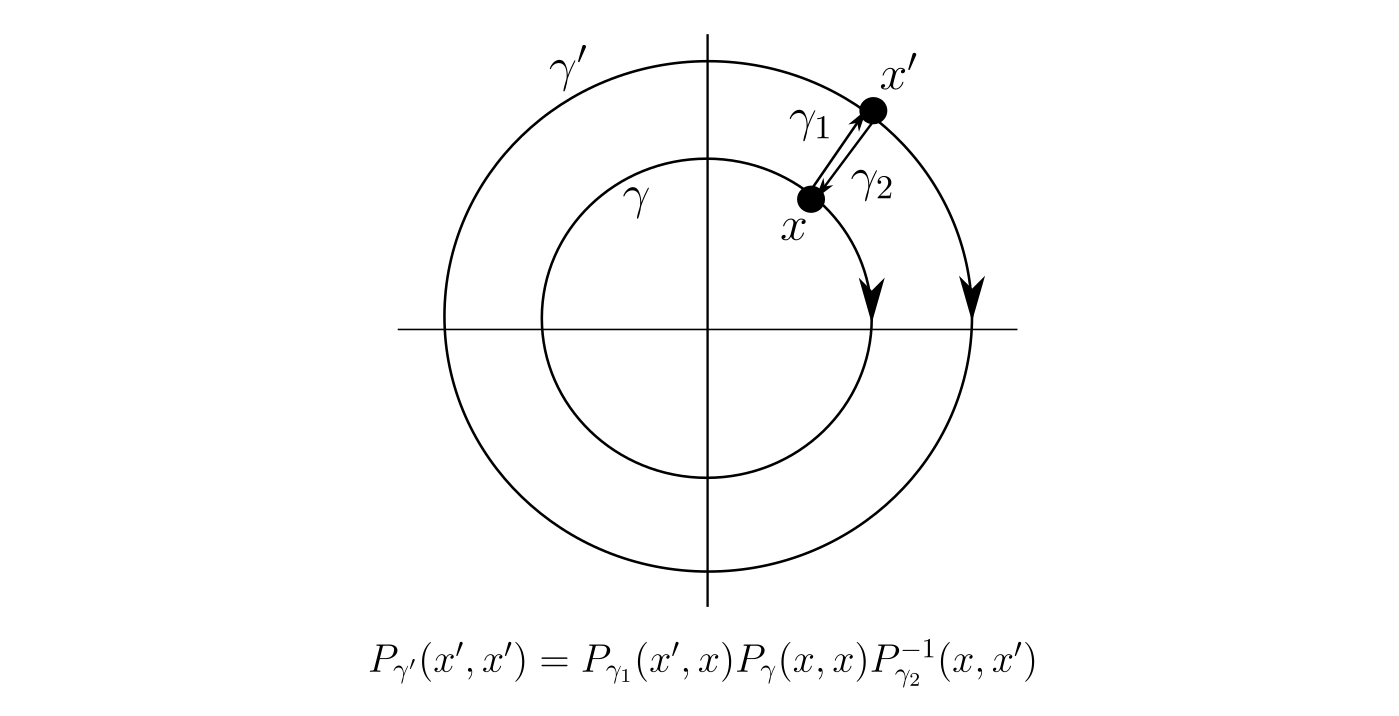
\includegraphics[width=\linewidth]{Figures/path_independence_gauge.png}
    \caption*{}
    \label{fig:31}
\end{figure}

So when $e^{i\xi}=1$, nothing happens when you move around a singularity - this means the wavefunction is unchanged! However, when $e^{i\xi}\neq 1$, you will be able to generate phases of $e^{i\xi n}$ for any $n \in \ZZ$ by transporting vectors around the singularity. This means that if you have some strange system with $e^{i\xi}\neq 1$ then dynamical effects will be observable due to the geometry of the system. This can only happen in two spacial dimensions!

\subsection{Free Particle in Two Dimensions}

Now let's consider the free particle in two dimensions. We will neglect center of mass coordinates, and use polar coordinates. The standard hamiltonian for a free particle in two dimensions is the following.

\begin{equation}
H = \frac{-1}{m}\left(\pdv[2]{r}+\frac{1}{r}\pdv{r}+ \frac{1}{r^2}\pdv[2]{\phi}\right)
\end{equation}

When you have this property that wavefunctions pick up a phase of $e^{i\xi}$ when you go around the singularity, you impose a nontrivial boundary condition: $\Psi(r,\phi+2\pi) = e^{i\xi}\Psi(r,\phi)$. This is what gives us strange dynamics - polar coordinates no longer gives us nice symmetry. There is, however, a transformation you can make to the Schrodinger equation that makes it easier to solve. The strategy is to replace $\Psi$ with $\Psi'(r,\phi) = e^{i\frac{\xi}{2\pi}\phi}\Psi(r,\phi)$. Then the Hamiltonian transforms as $H' = e^{-i\frac{\xi}{2\pi}\phi}H e^{i\frac{\xi}{2\pi}\phi}$. This gives $H\Psi = H'\Psi'$, so the solutions to the Schrodinger equation are unchanged. But observe what happens:

\begin{equation}
H' = \frac{-1}{m}\left(\pdv[2]{r}+\frac{1}{r}\pdv{r}+ \frac{1}{r^2}\left(\pdv{\phi}+\frac{i\xi}{2\pi}\right)^2\right)
\end{equation}

As an exercise, solve the Schrodinger equation after this transformation.

\subsection{Conclusions of Lecture 3}

This weirdness doesn't happen in three dimensions. The reason is that $\RP^{n-1}$ is doubly connected. Any curve $\gamma^2$ that goes around the singularity twice is contractible. Therefore we have $P_{\gamma^2}(x,x) = e^{2i\xi}=1$, so $\xi = 0$ or $\xi = \pi$. In the case that $\xi = \pi$, we have the dynamics of a fermion. In the case that $\xi = 0$ we have the dynamics of a boson! But what does it mean to go around the singularity once in $\RP^{n-1}$? It means you exchange the two particles. This is why fermions are antisymmetric under exchange, which is what causes the Pauli exclusion principle. We will see this in extreme detail in the following lectures.

\section{Prelim to Fock Space}
In the previous three lectures we've been looking at the quantum theory of identical particles in 3D. You can see what we've covered in these lectures as the tip of a very large iceberg, which we've only really begun to explore. What we have a good understanding of is the theory of identical point particles in 3 spacial dimensions or higher. What we have begun to uncover is the theory of extended, or membrane-like, interacting particles (ie, strings and so on). This falls under the title of "modular tensor categories". We will move on from this, but I wanted to make you aware before we move on that this field is still being studied extensively even now.

Another subject, very closely related - being the tip of this iceberg, is the study of Fock space and 'second quantization'. This is what we will cover for the next few lectures.

\subsection{Symmetric and Antisymmetric Representation}

We've learned about single particles in our elementary quantum mechanics course. What we would like to do is work out the Hilbert space to assign to a system of multiple particles provided that each of the particles has some Hilbert space of states $H$. Well, what we do know is the Hilbert space for N distinguishable particles, let's call it $\Hh$.
\begin{equation}
\Hh = H^{\otimes N} =: \bigotimes_{i=1}^N H
\end{equation}
But this space is too big to be what we want for indistinguishable particles. There are states in this space which would be physically the same. As an example, if you consider these to be position states of particles, then exchanging two particles would produce a positive or negative sign - in the case of a Boson there would be degeneracy here as the states would be identical.

We will use this information we learned - that $\ket{x_1,x_2} = \pm \ket{x_2, x_1}$ - and turn it into a way to reduce our Hilbert space to be something smaller. Of course, there is more information we could consider - such as when a particle has internal degrees of freedom such as spin. These are called parastatistics, but we won't cover them in this course.

The best way to reduce our model is to find a subspace of $\Hh$ which corresponds to exactly the unique configurations. There is a direct connection here between quantum theory and the representation theory of $S_N$ on $N$ symbols. This motivates us to define a representation.

\begin{defn}
Suppose $G$ is a group. A representation $U$ of $G$ over some vector space $V$ is a group homomorphism $U:G \to B(V)$, where $B(V)$ is the group of bounded linear operators on $V$.
\end{defn}

There are multiple definitions of a representation, but it doesn't matter here. We will focus on unitary representations since in this course we will usually consider transformations which correspond to unitary representations of some group. That is to say, we would like $U(g)$ to be unitary for any $g \in G$. There is a natural action of $S_N$ on $H^{\otimes N}$ given as follows.

\begin{equation}
U(\sigma)\ket{x_1,...,x_N} = \ket{x_{\sigma(1)},...,x_{\sigma(N)}}
\end{equation}

This action extends by linearity to our entire space (ie $U(\sigma)(a\ket{\psi}+b\ket{\phi}) = aU(\sigma)\ket{\psi}+bU(\sigma)\ket{\phi}$). What we should do, even though it is a tedious exercise, is write down a matrix for an example and see where that takes us.

Consider the permutation $\pi(1,2,3)=(3,1,2)$. We'd like to see the representation of this matrix on some space. Let's pick $\CC^2$ as our $H$, and $\Hh=H^{\otimes 3}$. Fix a basis $\ket{0},\ket{1}$ for the individual space. Then a basis for $\Hh$ is given as:
\[\ket{000},\ket{001},\ket{010},\ket{011},\ket{100},\ket{101},\ket{111}\]

Then a matrix representation for $\pi$ is given as follows.

\[U(\pi) =  \begin{bmatrix}
1&0&0&0&0&0&0&0\\
0&0&1&0&0&0&0&0\\
0&0&0&0&1&0&0&0\\
0&0&0&0&0&0&1&0\\
0&1&0&0&0&0&0&0\\
0&0&0&1&0&0&0&0\\
0&0&0&0&0&1&0&0\\
0&0&0&0&0&0&0&1
		\end{bmatrix}= \mathbb{I}\oplus
\begin{bmatrix}
0&1&0&0&0&0\\
0&0&0&1&0&0\\
0&0&0&0&0&1\\
1&0&0&0&0&0\\
0&0&1&0&0&0\\
0&0&0&0&1&0
\end{bmatrix}\oplus\mathbb{I}\]

You will notice that this matrix was block diagonal (to an extent). It is usually nice to look for bases where our matrices decompose into direct sums (or bases where our matrices can't be decomposed at all!). Such a choice of basis where matrices can't be decomposed into blocks (ie, a choice of representation associated with that basis) is called an irreducible representation. Let's move on now.

Since our particles are indistinguishable, there is no physically realizable experiment which could distinguish between two identical states. This means that for any observable $A$, we must have $U(\pi) A = A U(\pi)$ for all $\pi$. A very special role is played by vectors $\ket\psi$ such that $U(\pi) \ket{\psi} = \pm \ket{\psi}$. If we rewrite this in a peculiar way: $U(\pi)\ket{\psi} = u(\pi)\ket{\psi}$, you will see that this is an eigenvalue equation. We are searching for subspaces of $H^{\otimes N}$ which are simultaneous eigenspaces of all the permutation operators. The first thing we should argue is that this $u(\pi)$ is itself a representation of $S_N$ on $\CC$. We argue this because you will note that $U(\pi_1\pi_2) = u(\pi_1)u(\pi_2)$. Our claim is that there are only two distinct one-dimensional representations of the symmetric group. The proof is as follows.

Recall that every element of $S_N$ can be written as a product of other elements: $\pi = \tau_{ij} \circ ... \circ \tau_{k\ell}$ where each $\tau_{ij}$ is a 'transposition' (ie, for $\tau_{ij}(\ell)$ takes $i \to j$ and $j \to i$, and $\ell \to \ell$ if $j\neq \ell \neq i$). Thus we can deduce that for any one-dimensional representation of $S_N$ we have $u(\pi) = \prod_k u(\tau_{ij_k})$. This means that all one-dimensional representations are entirely characterized by the representations of the transpositions. We can try something else as well: note that $u(\pi)u(\tau_{ij})u(\pi^{-1}) = u(\pi\circ \tau_{ij}\circ \pi^{-1}) = u(\tau_{\pi(i)\pi(j)}) = u(\tau_{ij})$ (think about it for a minute). But for any $i,j$ there is some permutation so that $\pi(i,j) = (1,2)$! So we have completely characterized all representations by specifying $u(\tau_{12})$. We also know that $u(\tau_{12})^{2} = 1$, as transpositions are their own inverse, so there are only two possible solutions to this equation: $u(\tau_{12})=\pm1$. This completely determines all one-dimensional representations of $S_N$.
\begin{defn}[Trivial Representation]
The trivial 1D representation of $S_N$ is $u$ so that $u(\tau_{12}) = 1$. This means that $u(\pi) = 1$ for all $\pi \in S_N$.
\end{defn}
\begin{defn}[Antisymmetric Representation]
The antisymmetric representation of $S_N$ is $u$ so that $u(\tau_{12}) = -1$. This means that for any $\pi \in S_N$ we have $u(\pi) = \sgn(\pi)$.
\end{defn}

There is a fancy notation we can use in order to cover both cases at the same time - this way we don't need to always worry about which representation to deal with. Let's define $s$ as follows.
\[s(\pi)=\begin{cases}1 & u(\tau_{12})=1\\
\textrm{sgn}(\pi) & u(\tau_{12})=-1
\end{cases}\]
\pagebreak

\subsection{Antisymmetric/Symmetric Space}
Now that we have some machinery developed to study Bosons and Fermions, let's look at the following construction.
\begin{equation}
P_{+} = \frac{1}{N!}\sum_{\sigma \in S_N} U(\sigma)
\end{equation}
\begin{equation}
P_{-} = \frac{1}{N!}\sum_{\sigma \in S_N} \sgn(\sigma) U(\sigma)
\end{equation}
First of all, it's not clear what exactly these matrices are. What we see is that they are big sums of unitary matrices, but are they Hermitian? Unitary? What are they? We claim that these are both projections. That is: $P_{\pm}^2 = P_{\pm}$. We go through the proof of the first case, leaving the second as an exercise.
\[P_+^2 = \frac{1}{(N!)^2} \sum_{\pi,\pi'}U(\pi)U(\pi') = \frac{1}{(N!)^2}\sum_{\pi,\pi'} U(\pi \circ \pi')\]
Let $\sigma = \pi\circ \pi'$. Then we have:
\[P_+^2 = \frac{1}{(N!)^2} \sum_{\sigma,\pi^{-1}}U(\sigma) = \frac{1}{(N!)^2}\sum_{\sigma}U(\sigma) \sum_{\pi^{-1}}1 = \frac{1}{N!}\sum_{\sigma} U(\sigma) = P_+\]

Since these operators are projections, this tells us they have some associated invariant subspace $V$ where $P_\pm (V) = V$. Let's name these subspaces.
\begin{defn}[Symmetric/Antisymmetric Space]
We define the antisymmetric and the symmetric Hilbert spaces in the following formula.
\begin{equation}
\Hh_\pm^N = P_\pm(\Hh) = P_\pm(H^{\otimes N})
\end{equation}
\end{defn}
We see the following properties arise from these subspaces. Let $\ket{\psi} \in H_-^N$. Then $U(\tau_{12}) \ket{\psi} = U(\tau_{12}) \frac{1}{N!}\sum_{\pi}\sgn(\pi)U(\pi) \ket{\psi}$. So...
\[U(\tau_{12})\ket{\psi} = \frac{1}{N!}\sum_{\pi'}\sgn(\tau_{12}^{-1}\circ \pi')U(\pi') \ket{\psi} = \frac{1}{N!}\sum_{\pi'}\sgn(\tau_{12})\sgn(\pi')U(\pi')\ket{\psi}=-\ket{\psi}\] Similarly, for any $\psi \in \Hh_+^N$, $U(\pi)\ket{\psi} = \ket{\psi}$. This essentially gives us a way of defining Fermions and Bosons rigorously as elements of subspaces of an abstract Hilbert space.
\pagebreak
\section{Fock Space}
Before we begin this next section, let's introduce some shorthand notation.
\[H_s^N = \begin{cases}H_+^N & \textrm{ for bosons} \\ H_-^N & \textrm{ for fermions}\end{cases}\]
With $s = +1$ when we talk about Bosons and vice versa for Fermions.
\subsection{Definition of Fock Space}
Now we would like to generalize from a space with $N$ particles to a space with arbitrary numbers of particles. This way we can introduce or remove particles from our system. In fact, we can even allow $N$ itself to be a quantum number, and allow superpositions of states with differing numbers of particles! This leads to a process commonly known as Second Quantization whereby the notion of a 'particle' itself changes significantly. The space which allows this is called Fock Space, with the following definition.

\begin{defn}[Fock Space] We define the symmetric/antisymmetric Fock Space $\Gamma_s(\Hh)$ as the direct sum of all the individual Hilbert spaces.
\begin{equation}
\Gamma_s(\Hh) = \bigoplus_{N=0}^\infty \Hh_s^N =: \bigoplus_{N=0}^\infty \Gamma_{s,N}(\Hh)
\end{equation}
\end{defn}
Note that we define $H_s^0$ to be $H_s^0=:\CC$. This is the 'vacuum' space, with basis vector $\ket{\Omega}$, which is the vacuum state. It is the state of the system when there are no particles at all.

Recall that we can decompose a vector into it's components in a space. Let's do this for an arbitrary state $\ket{\psi} \in \Gamma_s(\Hh$. We see that $\ket{\psi} = \sum_{n=0}^\infty\sum_{i=0}^n \psi_n \ket{\phi_i}$, where each $\ket{\phi_i}$ is a basis vector from $\Gamma_{s,N}(\Hh)$. It is easy to see that $\Gamma_{s,N}(\Hh)$ is a separable space, but it remains to be shown that there is an inner product on this space. We will simply write $\ket{\psi} = \sum_{n=0}^\infty \ket{\psi_n}$ for the components of a vector in Fock space instead. Thus the scalar product on this space is $\braket{\psi}{\phi}=\sum_{n=0}^\infty \braket{\psi_n}{\phi_n}$. Now let's look at some observables on this space! What could we measure? The first one that comes to mind is the particle number operator $\hat N$.
\begin{defn}[Number Operator]
We define the particle number operator $\hat N$ as follows.
\begin{equation}
\hat N \ket{\psi_N} = N\ket{\psi_N} \forall \psi_N \in \Gamma_{s,N}(\Hh)
\end{equation}
\end{defn}
This way, states of determinate particle number are states where the only components are members of a subspace comprised of states with exactly $N$ particles. 

\subsection{Dynamics in Fock Space}
Now we would like to see what happens when we change the space according to some dynamics. That is, we want to look at maps $A : \Hh_1 \to \Hh_2$ and extend them to maps between different Fock spaces. This will allow us to define time evolution and so on. Well, we know how to produce from $A$ a linear operator from $\Hh_1^{\otimes N} \to \Hh_2^{\otimes N}$. We just tensor $A$ together $N$ times.
\[A^{\otimes N} : \Hh^{\otimes N}_1 \to \Hh_2^{\otimes N}\]
It turns out that the tensor product of operators respects antisymmetry and symmetry. That is to say, $A^{\otimes N}(\Gamma_{s,N}(\Hh_1)) = \Gamma_{s,N}(\Hh_2)$. You may recall this from previous studies of tensors. This comes from the fact that $[U(\pi),A^{\otimes N}] = 0$. We introduce some notation now.
\begin{equation}
\Gamma_{s}(A) : \Gamma_{s}(\Hh_1) \to \Gamma_s(\Hh_2)
\end{equation}
This definition is given by the following:
\begin{equation}
\Gamma_s(A) = \bigoplus_{N=0}^\infty \Gamma_{s,N}(A) =: \bigoplus_{N=0}^\infty A^{\otimes N}
\end{equation}
Where $\oplus$ here is the matrix direct sum.

\end{document}
